
\documentclass[12pt]{article}
\usepackage{enumitem}
\usepackage{geometry}
\usepackage{graphicx}
\geometry{margin=1in}

\title{TestRail Report – Snapshot 4}
\author{Haonan Ma}
\date{\today}

\begin{document}

\maketitle

\section*{Overview}
This document includes the results of Snapshot 4 testing for the LAPD1 Transcript Analysis System. Tests in this phase focused on UI/UX refinements, file validation, user notifications, session timeout handling, and role-based access control.

\section*{Snapshot Summary Image}
\begin{center}
    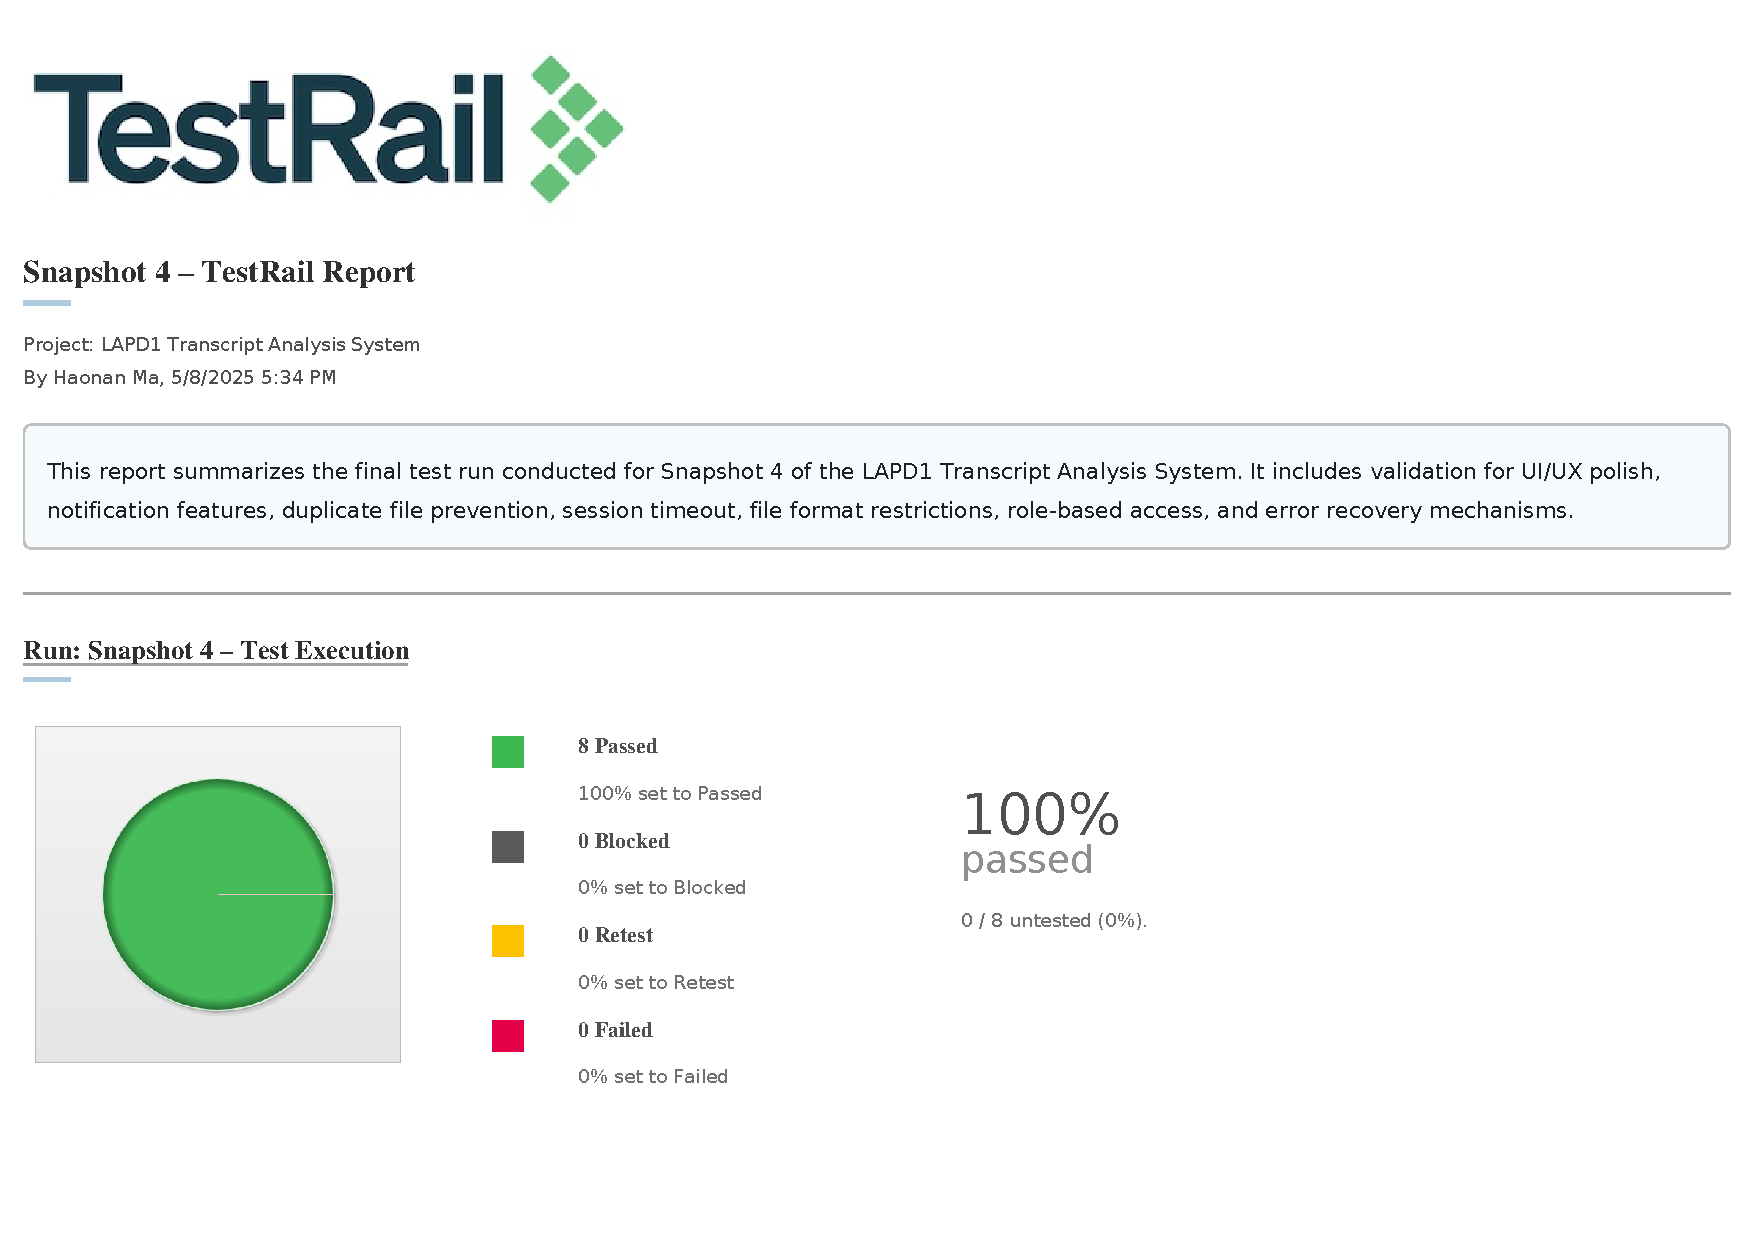
\includegraphics[width=\textwidth]{snapshot4image}
\end{center}

\section*{Test Cases}

\subsection*{Test Case 1: System Notification on Analysis Completion}
\textbf{Type:} Functional \\
\textbf{Priority:} Medium \\
\textbf{Estimate:} 3m \\
\textbf{Preconditions:} User is logged in and uploads a transcript for NLP analysis. \\
\textbf{Steps:}
\begin{enumerate}[label=\arabic*.]
\item Upload a transcript and start analysis.
\item Wait for the NLP process to complete.
\item Observe any in-app notification, toast, or modal.
\end{enumerate}
\textbf{Expected Result:} The system displays a real-time notification once processing finishes.

\subsection*{Test Case 2: Block Duplicate File Uploads}
\textbf{Type:} Functional \\
\textbf{Priority:} Medium \\
\textbf{Estimate:} 3m \\
\textbf{Preconditions:} A transcript has already been uploaded and analyzed. \\
\textbf{Steps:}
\begin{enumerate}[label=\arabic*.]
\item Upload a transcript file (e.g., “evidence1.pdf”) and complete analysis.
\item Attempt to upload the same file again.
\item Observe the system response.
\end{enumerate}
\textbf{Expected Result:} The system blocks duplicate submissions and shows a warning.

\subsection*{Test Case 3: Dark Mode UI Toggle}
\textbf{Type:} Functional \\
\textbf{Priority:} Low \\
\textbf{Estimate:} 2m \\
\textbf{Preconditions:} User is logged in and on any main interface screen. \\
\textbf{Steps:}
\begin{enumerate}[label=\arabic*.]
\item Locate and click the “Dark Mode” toggle switch.
\item Wait for UI theme update.
\item Interact with the interface.
\item Toggle back to light mode.
\end{enumerate}
\textbf{Expected Result:} Theme switches properly and UI elements remain usable.

\subsection*{Test Case 4: Show Error for Unsupported File Type (.exe)}
\textbf{Type:} Security \\
\textbf{Priority:} High \\
\textbf{Estimate:} 2m \\
\textbf{Preconditions:} Encrypted (password-protected) document is ready. \\
\textbf{Steps:}
\begin{enumerate}[label=\arabic*.]
\item Select a file with the `.exe` extension.
\item Click “Analyze” to attempt upload.
\item Observe the system response.
\end{enumerate}
\textbf{Expected Result:} The system blocks the upload and shows an error.

\subsection*{Test Case 5: Session Timeout Auto-Logout}
\textbf{Type:} Security \\
\textbf{Priority:} Medium \\
\textbf{Estimate:} 7m \\
\textbf{Preconditions:} User is logged in and leaves the session idle. \\
\textbf{Steps:}
\begin{enumerate}[label=\arabic*.]
\item Log in and remain idle.
\item Wait for timeout period.
\item Observe system behavior.
\end{enumerate}
\textbf{Expected Result:} System logs the user out and redirects to login page.

\subsection*{Test Case 6: Save and Resume Draft Upload}
\textbf{Type:} Functional \\
\textbf{Priority:} Medium \\
\textbf{Estimate:} 5m \\
\textbf{Preconditions:} Upload process or metadata form is started. \\
\textbf{Steps:}
\begin{enumerate}[label=\arabic*.]
\item Begin uploading a file or filling out metadata.
\item Refresh or navigate away.
\item Return to the page.
\end{enumerate}
\textbf{Expected Result:} Previously entered content and uploads are preserved.

\subsection*{Test Case 7: Role-Based Admin Access Control}
\textbf{Type:} Security \\
\textbf{Priority:} High \\
\textbf{Estimate:} 5m \\
\textbf{Preconditions:} Multiple user roles exist: viewer, editor, admin. \\
\textbf{Steps:}
\begin{enumerate}[label=\arabic*.]
\item Try accessing admin panel with each role.
\item Observe access control behavior.
\end{enumerate}
\textbf{Expected Result:} Only admin users can access admin panel. Others are denied.

\subsection*{Test Case 8: Email Notification on Failed Analysis}
\textbf{Type:} Functional \\
\textbf{Priority:} Medium \\
\textbf{Estimate:} 6m \\
\textbf{Preconditions:} Corrupted or invalid transcript file is available. \\
\textbf{Steps:}
\begin{enumerate}[label=\arabic*.]
\item Upload a problematic file.
\item Trigger analysis failure.
\item Check email inbox.
\end{enumerate}
\textbf{Expected Result:} System sends an email with failure reason and details.

\end{document}
